\documentclass[12pt]{article}
\usepackage[svgnames,x11names,table]{xcolor}
\usepackage{hyperref}
\usepackage{graphicx}
\usepackage{parskip}
\usepackage{float}
\usepackage{amsmath}
\usepackage{amssymb}
\usepackage{enumitem}
\usepackage[thicklines]{cancel}

\hypersetup{
    colorlinks,
    citecolor=black,
    filecolor=black,
    linkcolor=RoyalBlue4,
    urlcolor=RoyalBlue4,
}

\title{PEU 453 Assignment 5}
\author{Mohamed Hussien El-Deeb (201900052)}
\date{}

\begin{document}

\maketitle
\tableofcontents

\renewcommand{\labelenumi}{\textbf{\alph{enumi}.}}

\newpage

\section{Problem 5.3}

 (Do problem 5.1 first.) Consider the coordinate basis discussed in box 5.1 for polar coordinates \(r, \theta \).

\begin{enumerate}
      \item Consider an object moving at a constant speed \(v\) in the \(+y\) direction of the cartesian coordinate system, so that \(v^y=v, v^z=0\). Find the components \(v^r\) and \(v^\theta \) of this object's velocity in the polar coordinate system. Express your results both purely in terms of \(r\) and \(\theta \) and purely in terms of \(x\) and \(y\).
      \item Imagine that the object starts at \(x=b, y=0\) at time \(t=0\). Its subsequent \(y\) position at later times \(t\) will therefore be simply \(y=v t\). Use this to express both the object's \(r\) and \(\theta \) position and its polar coordinate velocity components \(v^r\) and \(v^\theta \) at all times \(t>0\) in terms of \(v\), \(b, r\), and \(t\). Does your result make sense? (In particular, if you sketch the object's path, you should be able to see that its velocity will be mostly in the \(\theta \) direction at early times, but mostly in the \(r\) direction at late times. Is this consistent with your mathematical expressions?)
\end{enumerate}

\textbf{a.}

\begin{equation*}
      \begin{split}
            {\Lambda_\mu}^\nu
             & = \frac{\partial x^\nu}{\partial {x'}^\mu}                                                   \\
             & =
            \begin{bmatrix}
                  \frac{\partial x}{\partial r}      & \frac{\partial y}{\partial r}      \\
                  \frac{\partial x}{\partial \theta} & \frac{\partial y}{\partial \theta} \\
            \end{bmatrix}                         \\
             & =
            \begin{bmatrix}
                  \frac{\partial (r \cos{\theta}) }{\partial r}      & \frac{\partial (r \sin{\theta}) }{\partial r}      \\
                  \frac{\partial (r \cos{\theta}) }{\partial \theta} & \frac{\partial (r \sin{\theta}) }{\partial \theta} \\
            \end{bmatrix} \\
             & =
            \begin{bmatrix}
                  \cos{\theta}     & \sin{\theta}   \\
                  - r \sin{\theta} & r \cos{\theta} \\
            \end{bmatrix}
      \end{split}
\end{equation*}

\[
      \mathbf{v} =
      \begin{bmatrix}
            0 \\
            v \\
      \end{bmatrix}
\]

\begin{equation*}
      \begin{split}
            {\mathbf{v}'}_\mu
             & =
            {\Lambda_\mu}^\nu \mathbf{v}_\nu \\
             & =
            \begin{bmatrix}
                  \cos{\theta}     & \sin{\theta}   \\
                  - r \sin{\theta} & r \cos{\theta} \\
            \end{bmatrix}
            \begin{bmatrix}
                  0 \\
                  v \\
            \end{bmatrix}                   \\
             & = v
            \begin{bmatrix}
                  \sin{\theta}   \\
                  r \cos{\theta} \\
            \end{bmatrix}                   \\
             & = v
            \begin{bmatrix}
                  \frac{y}{\sqrt{x^2+y^2}} \\
                  x                        \\
            \end{bmatrix} \\
      \end{split}
\end{equation*}

\[
      g^{\mu \nu} =
      \begin{bmatrix}
            1 & 0             \\
            0 & \frac{1}{r^2} \\
      \end{bmatrix}
\]

\[
      {\mathbf{v}'}^\mu = g^{\mu\nu} {\mathbf{v}'}_\nu
\]

\[
      {\mathbf{v}'}^i
      = v
      \begin{bmatrix}
            \sin{\theta}           \\
            \frac{\cos{\theta}}{r} \\
      \end{bmatrix}                   \\
      = v
      \begin{bmatrix}
            \frac{y}{\sqrt{x^2+y^2}} \\
            \frac{x}{x^2+y^2}        \\
      \end{bmatrix} \\
\]

\textbf{b.}

\[
      \mathbf{r} =
      \begin{bmatrix}
            b  \\
            vt \\
      \end{bmatrix}
\]

\[
      \mathbf{r}' =
      \begin{bmatrix}
            r \\
            0 \\
      \end{bmatrix} = \begin{bmatrix}
            \sqrt{b^2+v^2t^2} \\
            0                 \\
      \end{bmatrix}
\]

\[
      \theta = \tan^{-1}{(\frac{y}{x})} = \tan^{-1}{(\frac{vt}{b})}
\]

\[
      {\mathbf{v}'}^i
      = v
      \begin{bmatrix}
            \frac{vt}{\sqrt{b^2+v^2t^2}} \\
            \frac{b}{b^2+v^2t^2}         \\
      \end{bmatrix} \\
\]

\[
      \lim_{t \rightarrow 0}[v] = \begin{bmatrix}
            0 \\
            v \\
      \end{bmatrix}
\]

\[
      \lim_{t \rightarrow \infty}[v] = \begin{bmatrix}
            v \\
            0 \\
      \end{bmatrix}
\]

Yes it is consistent

\newpage

\section{Problem 5.5}

We can define ``sinusoidal'' coordinates \(u, w\) on a flat 2D plane by the relations \(u=x\) and \(w=y-A \sin (b x)\), where \(A\) and \(b\) are constants. For the sake of concreteness, let \(A=1.0 \mathrm{~cm}\) and \(b=\pi / 2 \mathrm{~cm}^{-1}\).

\begin{enumerate}
      \item Sketch what the ``curves'' of constant \(u\) and constant \(w\) look like in a cartesian \(x, y\) coordinate system.
      \item What is the metric of the sinusoidal coordinate system? Is this metric diagonal?
      \item Imagine that an object moves with constant velocity \(\boldsymbol{v}\) such that \(v^x=v\) and \(v^y=0\). Such an object's position will be \(x=v t\) (assuming \(x=0\) at \(t=0\)) and \(y=\) constant. Find the object's velocity components \(v^\mu \) and \(v^w\) in the \(u, w\) coordinate system. Express your results in terms of \(v, t, A\), and \(b\).
      \item Show that the squared magnitude of \(\boldsymbol{v}\) is still the constant \(v^2\) in this coordinate system, even though the velocity component \(V^w\) is not constant in time. Explain why \(V^w\) is not constant, even though the vector \(v\) in abstract always points in the same direction and always has the same magnitude.
      \item Argue therefore that \(d v^w / d t\) cannot be equal to the component \(a^w\) of the object's acceleration vector \(\boldsymbol{a}\) in the \(u\), \(w\) coordinate system. (Hint: Note that \(a^w=a^y=0\) in the cartesian system.) We will learn in a later chapter how to take derivatives correctly in an curvilinear coordinate system.
\end{enumerate}

\textbf{a.}

\begin{figure}[H]
      \centering
      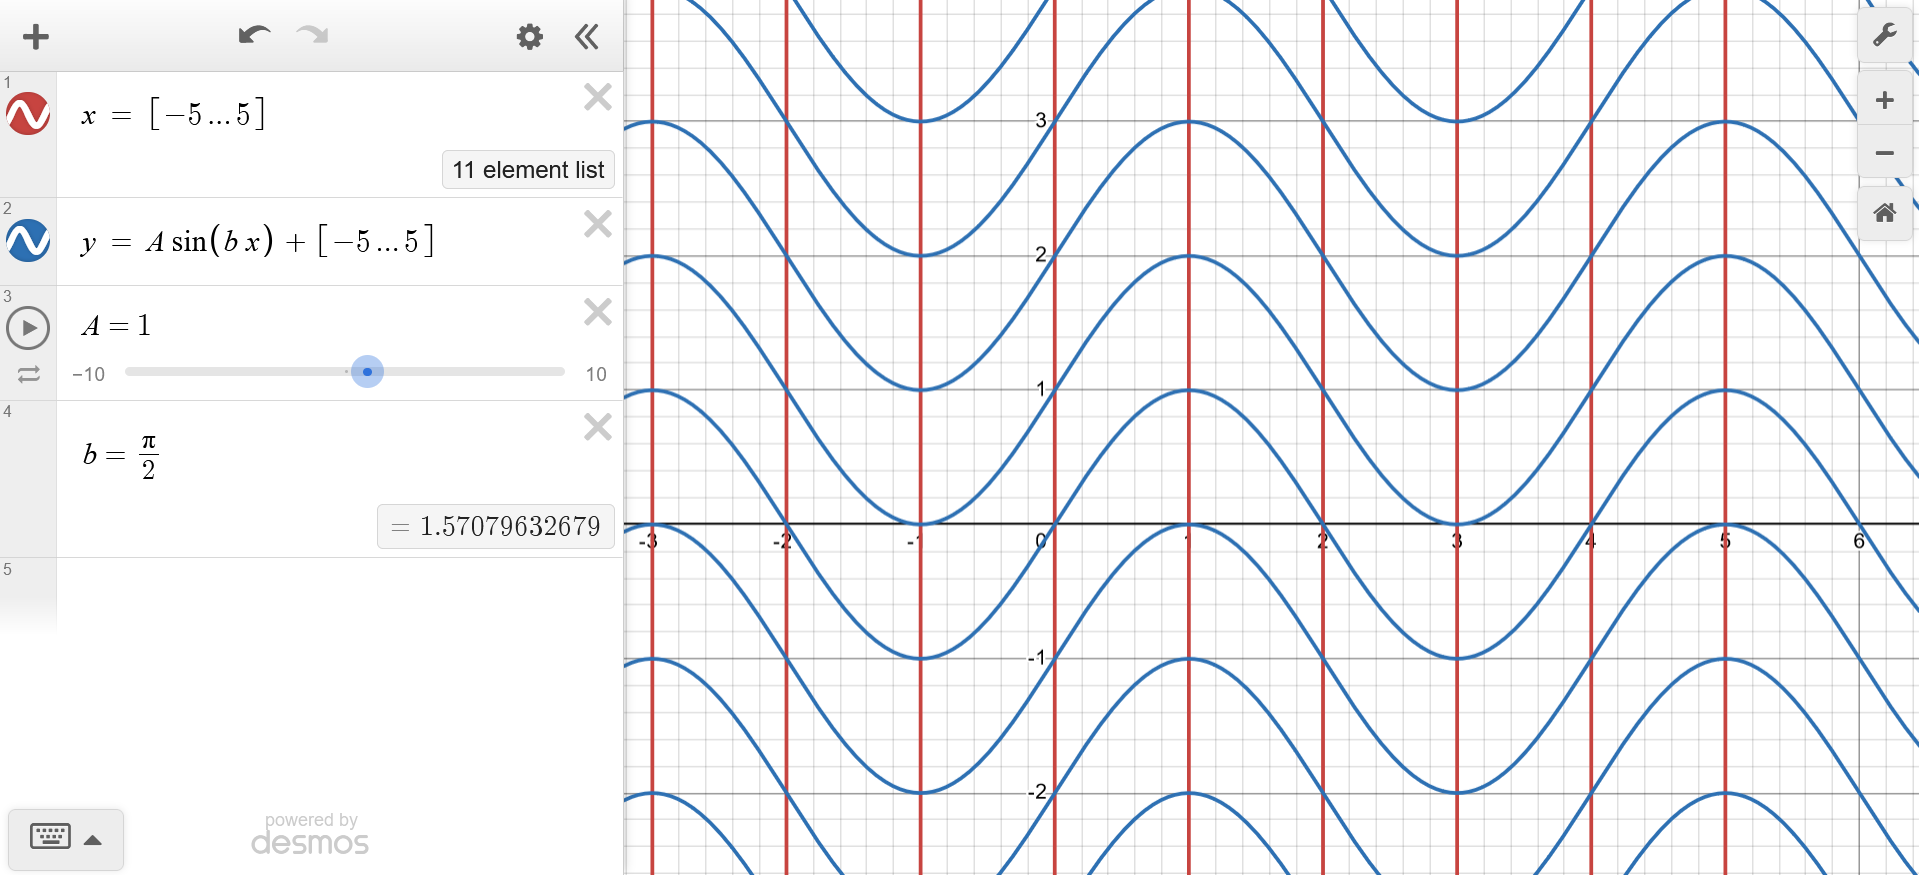
\includegraphics[scale=0.15]{Q2.png}
\end{figure}

\textbf{b.}

\[
      x = u,\quad y = w + \sin(\frac{\pi}{2} u)
\]

\[
      g'_{\mu\nu} = \frac{\partial x^\alpha}{\partial x'^\mu} \frac{\partial x^\beta}{\partial x'^\nu} g_{\alpha\beta}
\]

\[
      g'_{\mu\nu} = \frac{\partial x^\alpha}{\partial x'^\mu} \frac{\partial x^\beta}{\partial x'^\nu} \delta_{\alpha\beta}
\]

\[
      \frac{\partial x}{\partial u} = 1, \quad \frac{\partial x}{\partial w} = 0
\]

\[
      \frac{\partial y}{\partial u} = \frac{\pi}{2} \cos(\frac{\pi}{2}u), \quad \frac{\partial y}{\partial w} = 1
\]

\[
      g_{u u} = {(\frac{\partial x^\alpha}{\partial u})}^2 =
      {(\frac{\partial x}{\partial u})}^2 + {(\frac{\partial y}{\partial u})}^2=
      1 + {(\frac{\pi}{2} \cos(\frac{\pi}{2}u))}^2
\]

\[
      g_{u w} = \frac{\partial x^\alpha}{\partial x^u} \frac{\partial x^\alpha}{\partial x^w} =
      \frac{\partial x}{\partial u} \frac{\partial x}{\partial w} + \frac{\partial y}{\partial u} \frac{\partial y}{\partial w} =
      \frac{\pi}{2} \cos(\frac{\pi}{2}u)
\]

\[
      g_{u w} =  g_{w u}
\]

\[
      g_{w w} = {(\frac{\partial x^\alpha}{\partial w})}^2 =
      {(\frac{\partial x}{\partial w})}^2 + {(\frac{\partial y}{\partial w})}^2=
      1
\]

It is not diagonal

\textbf{c.}

\[
      {\Lambda^\mu}_\nu = \frac{\partial {x'}^\mu}{\partial x^\nu}
\]

\[
      \frac{\partial u}{\partial x} = 1, \quad \frac{\partial w}{\partial x} = -\frac{\pi}{2} \cos(\frac{\pi}{2}x)
\]

\[
      \frac{\partial u}{\partial y} = 0, \quad \frac{\partial w}{\partial y} = 1
\]

\[
      \Lambda = \begin{bmatrix}
            1                                   & 0 \\
            -\frac{\pi}{2} \cos(\frac{\pi}{2}x) & 1 \\
      \end{bmatrix}
\]

\[
      \mathbf{v} =
      \begin{bmatrix}
            v \\
            0 \\
      \end{bmatrix}
\]

\[
      \mathbf{v}' =
      \begin{bmatrix}
            1                                   & 0 \\
            -\frac{\pi}{2} \cos(\frac{\pi}{2}x) & 1 \\
      \end{bmatrix}\begin{bmatrix}
            v \\
            0 \\
      \end{bmatrix} =
      v \begin{bmatrix}
            1                                   \\
            -\frac{\pi}{2} \cos(\frac{\pi}{2}x) \\
      \end{bmatrix}
\]

\textbf{d.}

\[
      g = \begin{bmatrix}
            1 + {(\frac{\pi}{2} \cos(\frac{\pi}{2}u))}^2 & \frac{\pi}{2} \cos(\frac{\pi}{2}u) \\
            \frac{\pi}{2} \cos(\frac{\pi}{2}u)           & 1                                  \\
      \end{bmatrix}
\]


\[
      \mathbf{v}' \cdot \mathbf{v}'= g_{i j} {(\mathbf{v}')}^i {(\mathbf{v}')}^j
\]

\[
      = g_{u u} {({(\mathbf{v}')}^u)}^2
      + g_{w u} {(\mathbf{v}')}^u {(\mathbf{v}')}^w
      + g_{u w} {(\mathbf{v}')}^w {(\mathbf{v}')}^u
      + g_{w w} {({(\mathbf{v}')}^w)}^2
\]

\[
      = (1 + {(\frac{\pi}{2} \cos(\frac{\pi}{2}u))}^2)v^2
      - 2 {(\frac{\pi}{2} \cos(\frac{\pi}{2}x))}^2 v^2
      + {(\frac{\pi}{2} \cos(\frac{\pi}{2}x))}^2 v^2
\]

\[
      = (1 + {(\frac{\pi}{2} \cos(\frac{\pi}{2}u))}^2)v^2
      - {(\frac{\pi}{2} \cos(\frac{\pi}{2}x))}^2 v^2
\]

\[
      = v^2
\]

\[
      \mathbf{v} \cdot \mathbf{v} = v^2
\]

$V'$ is not constant since the new coordinates themselves are not constant so any constant will be a function of space.

\textbf{e.}

\[
      \mathbf{v}' =
      v \begin{bmatrix}
            1                                     \\
            -\frac{\pi}{2} \cos(\frac{\pi}{2}v t) \\
      \end{bmatrix}
\]


\[
      \frac{d v^w}{d t} = -v\frac{\pi}{2} \frac{d (\cos(\frac{\pi}{2}v t))}{d t}
      = {(v\frac{\pi}{2})}^2 \sin(\frac{\pi}{2}v t)
\]

Since a is zero in cartesian it will be 0 in the new coordinate system which is not the same.

\newpage

\section{Problem 5.7}

Consider the two-dimensional surface of a paraboloid defined by the relation \(z=b r^2\) (where \(b\) is some constant and \(r^2=x^2+y^2\)) in a 3D flat (Euclidean) space.

\begin{enumerate}
      \item Sketch this surface in a 3D \(x y z\) plot.
      \item Define coordinates \(r, \phi \) for this surface, where the \(r\) coordinate of a point on the surface is defined as above and \(\phi \) is an angle measured around the surface's axis of symmetry (the \(z\) axis), like a longitudinal coordinate on the earth. Determine the metric components \(g_{\mu v}\) for these coordinates on the paraboloid's surface, assuming that we use a coordinate basis. (Hint: Note that a step toward larger \(r\) on the surface means not only moving away from the \(z\) axis in the 3D space but also moving upward to more positive z. What is the distance \(d s\) along the surface involved in a step of \(d r\) along a curve of constant \(\phi \))?
\end{enumerate}

\textbf{a.}

\begin{figure}[H]
      \centering
      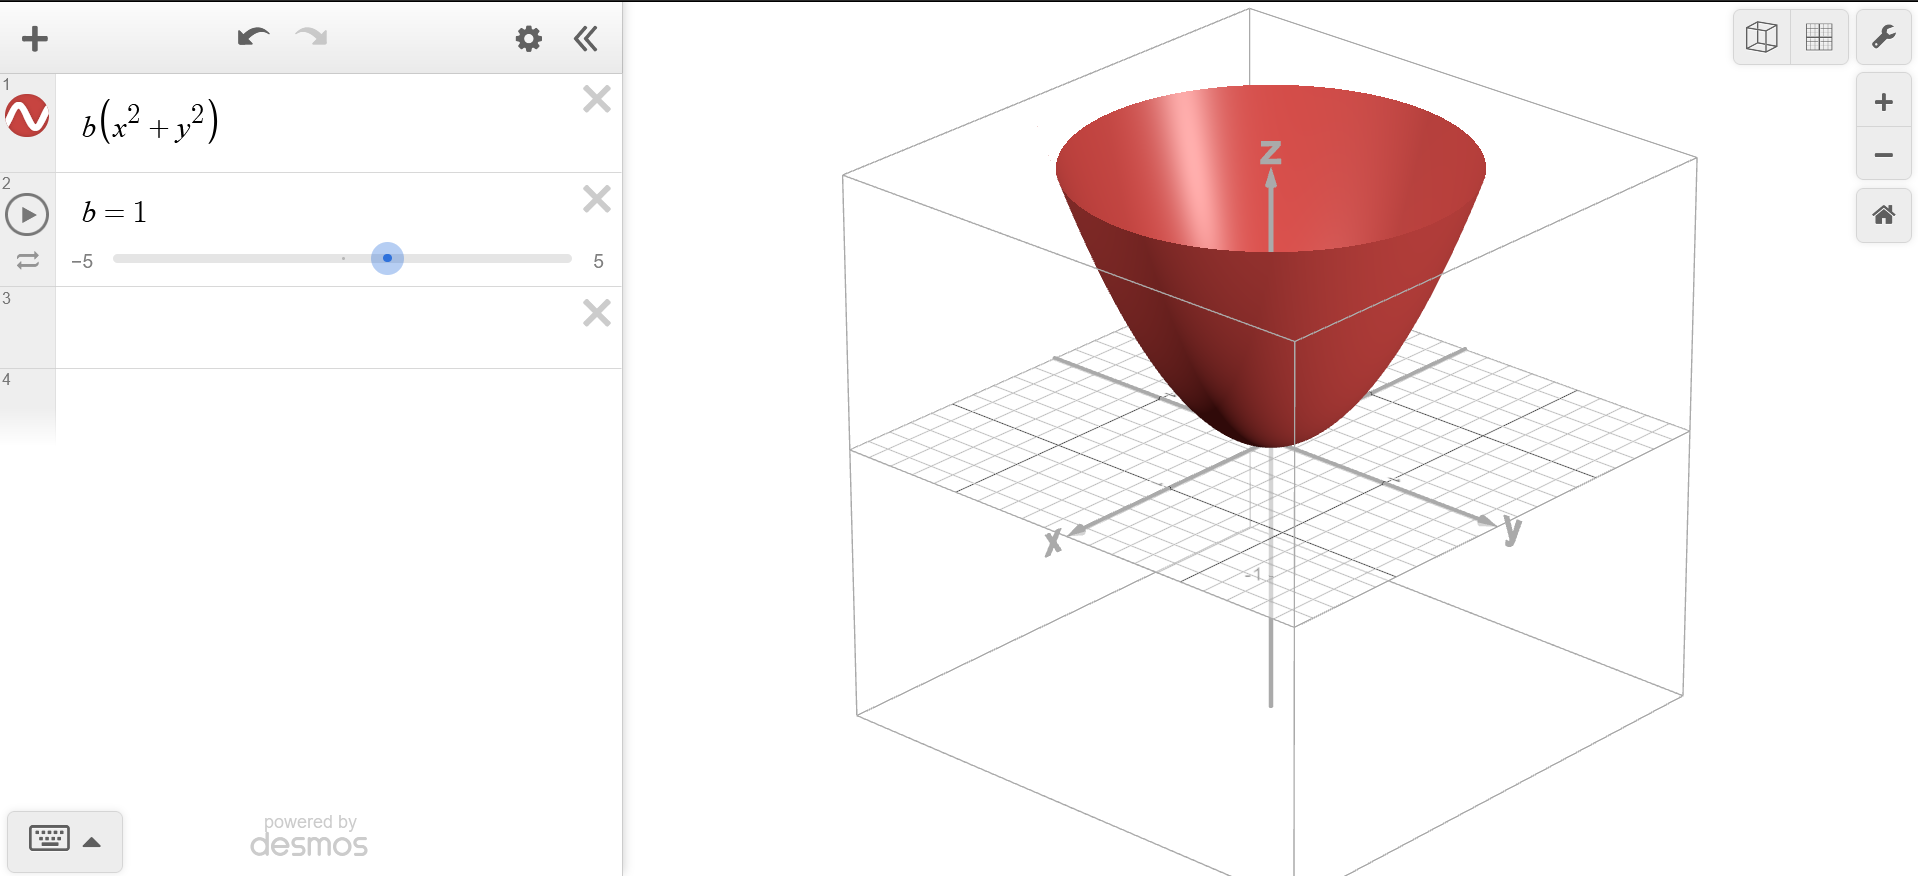
\includegraphics[scale=0.15]{Q3.png}
\end{figure}

\textbf{b.}

\[
      r = \sqrt{x^2+y^2}, \quad \phi = \tan^{-1}(\frac{y}{x}), \quad z = b (x^2+y^2)
\]
\[
      x = r\cos{\phi}, \quad y = r\sin{\phi}, \quad z = br^2
\]

\[
      g'_{\mu\nu} = \frac{\partial x^\alpha}{\partial x'^\mu} \frac{\partial x^\beta}{\partial x'^\nu} \delta_{\alpha\beta}
\]


\begin{equation*}
      g'_{\mu \nu} =
      \begin{bmatrix}
            g'_{r r}    & g'_{r \phi}    & g'_{r z}    \\
            g'_{\phi r} & g'_{\phi \phi} & g'_{\phi z} \\
            g'_{z r}    & g'_{z \phi}    & g'_{z z}
      \end{bmatrix}
\end{equation*}

\begin{equation*}
      \begin{split}
            g'_{r r} & = {\left(\frac{\partial x}{\partial r} \right)}^2 +
            {\left(\frac{\partial y}{\partial r} \right)}^2 +
            {\left(\frac{\partial z}{\partial r} \right)}^2                \\
                     & = \cos^2\phi + \sin^2\phi + (2br)^2                 \\
                     & = 1 + 4b^2r^2
      \end{split}
\end{equation*}

\begin{equation*}
      \begin{split}
            g'_{\phi r} = g'_{r \phi} & =
            \frac{\partial x^\alpha}{\partial r} \frac{\partial x^\beta}{\partial \phi} \delta_{\alpha\beta}                                                                                                                               \\
                                      & = \frac{\partial x}{\partial r} \frac{\partial x}{\partial \phi} + \frac{\partial y}{\partial r} \frac{\partial y}{\partial \phi} + \frac{\partial z}{\partial r} \frac{\partial z}{\partial \phi} \\
                                      & = (\cos\phi)(-r \sin\phi) + (\sin\phi)(r\cos\phi) + 0                                                                                                                                              \\
                                      & = 0
      \end{split}
\end{equation*}

\begin{equation*}
      \begin{split}
            g'_{z r} = g'_{r z} & =
            \frac{\partial x^\alpha}{\partial r} \frac{\partial x^\beta}{\partial z} \delta_{\alpha\beta}                                                                                                                   \\
                                & = \frac{\partial x}{\partial r} \frac{\partial x}{\partial z} + \frac{\partial y}{\partial r} \frac{\partial y}{\partial z} + \frac{\partial z}{\partial r} \frac{\partial z}{\partial z} \\
                                & = 0 + 0 + 2br                                                                                                                                                                             \\
                                & = 2br
      \end{split}
\end{equation*}

\begin{equation*}
      \begin{split}
            g'_{\phi \phi} & = {\left(\frac{\partial x}{\partial \phi} \right)}^2 +
            {\left(\frac{\partial y}{\partial \phi} \right)}^2 +
            {\left(\frac{\partial z}{\partial \phi} \right)}^2                      \\
                           & = (-r\sin\phi)^2 + (r\cos\phi)^2 + 0                   \\
                           & = r^2\sin^2\phi + r^2\cos^2\phi                        \\
                           & = r^2
      \end{split}
\end{equation*}

\begin{equation*}
      \begin{split}
            g'_{\phi z} = g'_{z \phi} & =
            \frac{\partial x^\alpha}{\partial z} \frac{\partial x^\beta}{\partial \phi} \delta_{\alpha\beta}                                                                                                                               \\
                                      & = \frac{\partial x}{\partial z} \frac{\partial x}{\partial \phi} + \frac{\partial y}{\partial z} \frac{\partial y}{\partial \phi} + \frac{\partial z}{\partial z} \frac{\partial z}{\partial \phi} \\
                                      & = 0 + 0 + 0                                                                                                                                                                                        \\
                                      & = 0
      \end{split}
\end{equation*}

\begin{equation*}
      \begin{split}
            g'_{z z} & = {\left(\frac{\partial x}{\partial z} \right)}^2 +
            {\left(\frac{\partial y}{\partial z} \right)}^2 +
            {\left(\frac{\partial z}{\partial z} \right)}^2                \\
                     & = 0 + 0 + 1                                         \\
                     & = 1
      \end{split}
\end{equation*}
\begin{equation*}
      g'_{\mu\nu} =
      \begin{bmatrix}
            1 + 4b^2r^2 & 0   & 2br \\
            0           & r^2 & 0   \\
            2br         & 0   & 1
      \end{bmatrix}
\end{equation*}
For a step of \(dr\) along a curve of constant \(\phi\)
\[dz = \frac{dz}{dr}dr = 2br\, dr\]
\begin{equation*}
      \begin{split}
            ds^2 & = g'_{\mu \nu} dx^\mu dx^\nu                                   \\
                 & = g'_{r r}\,dr^2 + 2g_{r z}\,dr dz + g_{z z}\,dz^2             \\
                 & = g'_{r r}\,dr^2 + 2(2br)g_{r z}\,dr^2 + (2br)^2 g_{z z}\,dr^2 \\
                 & = \left[(1 + 4b^2r^2) + 2(2br)^2 + (2br)^2\right] dr^2         \\
                 & = (1+ 16 b^2r^2)\, dr^2
      \end{split}
\end{equation*}

\[
      ds = \sqrt{1+ 16 b^2r^2}\, dr
\]


\newpage

\bibliographystyle{plain}
\bibliography{references}
\nocite{El-Deeb_PEU-453_Assignments}

\end{document}